\chapter{Pulse Generation by an XFEL}
X-ray Free-electron lasers (XFELs) can generate multi gigawatt and femtosecond (fs) x-ray radiation. Compared to fourth-generation synchrotrons, this is a ten billion-fold increase in brightness. Typically an XFEL consists of two main structures: a linear accelerator, and an undulator. The X-ray radiation is generated in the undulator.  This chapter describes the operation of both structures. 

\section{The linear accelerator}

At the beginning of the linear acceleration, an electron gun releases short bunches of electrons. The electron bunches are accelerated to relativistic energies, using the electric fields generated by radio frequency (RF) amplifiers named klystrons. Each klystron can maximally add 30 MW/m of energy to the electron bunch. Under higher currents the klystron will tear itself apart. In order to reach sufficiently energetic electron bunches, the linear accelerator are typically hundreds of meters up to close to a kilometre long.

Often accelerators do not operate at the point of maximum acceleration, since one wants to introduce a negative energy gradient along the particle bunch that can later be utilized for bunch compression. This acceleration method is called off-crest acceleration, and is visualized in figure  \ref{fig:AC}. A negative energy gradient means that the electrons located at the front of the bunch have a slightly lower energy compared to the electrons located at the rear of the bunch.

\begin{figure}[h]
\centering
\includegraphics[width=100mm]{Chapter_03_Acceleration_v2.png}
\caption{Schematic of acceleration and bunch compression at LCLS. a-c) change of bunch shape throughout the accelerator. d) illustration of the off-crest accelleration principle. a) shows that this creates an energy chirp. e) schematic of a single klystron. f) schematic of a chicane. The green and red blocks represent magnetic dipoles that deflect the electron bunch in the opposite direction. The path of high energy electrons diverges less than lower energy electrons. If the bunch has a negative energy chirp, this results in bunch compression.}\label{fig:AC}
\end{figure}

\subsection{Bunch Compression}
Short and compact bunches are essential for an XFEL. The main bunch-compression devices are chicanes. Chicanes consist of four magnetic dipoles that cause the high energy part of the bunch to deflect less than the low energy part (see Figure \ref{fig:AC} ). Due to the negative energy gradient it thus reduces the temporal spread of the bunch. After the final compression the electron bunch is ~40 fs long. Creating these short bunches is a noteworthy technical achievement.


The intensity of this radiation scales with the number of electrons in the bunch. Photons co-propagate with the relativistic electrons and if the undulator is long enough, induce an energy modulation, leading to a periodic density modulation in the electron cloud. The resulting microbunches behave like giant charged particles, and emit photons proportional to the square of their total charge in the undulator. At wavelengths longer than the bunch length, this radiation is coherent. This phenomenon of self-amplified spontaneous emission (SASE) is exploited to create powerful X-ray free-electron lasers, using very long undulator structures.




\section{Undulator}
After the acceleration the electron bunches are sent through a periodic arrangement of magnets with alternating poles called an undulator. The magnetic field in the undulator is given by:
\begin{equation}\vec{B}(z) = B_0\cos{(\frac{2\pi}{\lambda_u}z)}\hat{\mathbf{y}}\label{eq:bz}\end{equation}
where $B_0$ is the magnetic field and $\lambda_u$ is the length of an undulator period.
Due to the magnetic field the moving bunch of electrons experience a Lorentz force, causing it to oscillate in the transverse direction (x). The movement can be described by the following equation. 
%\begin{equation}\vec{F} = e(\vec{v}\times\vec{B})\end{equation}
\begin{equation}v_x = \frac{-e\,B_0\,\lambda_u}{2\pi\,m_e\gamma} \sin{(\frac{2\pi}{\lambda_u}z)} = \frac{K c}{\gamma} \sin{(k_uz)}\label{eq:vx}\end{equation}
The non-dimensional parameter K is given by:
\[K =  \frac{-e\,B_0\,\lambda_u}{2\pi\,m_e \, c}  \approx 0.9337 B_0 \lambda_u\]
where the approximation is valid when the magnetic field is given in Tesla and the undulator period in centimeters.

To preserve momentum during the oscillation, the electrons emit radiation with a wavelength $\lambda_s$. As described in Chapter 2, interference effects will occur between the emitted waves from the different electrons. The essence of this interference phenomenon lies in the longer route taken by the oscillating electrons compared to the radiation, which causes an OPD between the radiation emitted by electrons one undulator period apart. If the OPD between the electrons and the radiation is equal to a multiple of $\lambda_s$, the emitted waves will add coherently. Radiation with other wavelengths will interfere destructively. The longer an undulator, the more pronounced will this selection of specific wavelengths be. Equation \ref{eq:res} describes this so-called resonance condition.%, as shown in figure 3b.
\begin{equation}c\frac{\lambda_u}{\langle v_z \rangle } -\lambda_u\, \cos{(\theta)} = n \lambda_s \label{eq:res}\end{equation}
To predict at which wavelength this happens we need to find the average longitudinal velocity $\langle v_z \rangle$. Since the total speed, $v$, of the electrons is not affected by the Lorentz force, the longitudinal speed is calculated using pythagoras theorem: $v_z = \sqrt{ {v}^2-{v_x}^2}$. Using Equation \ref{eq:vx} for $v_x$ and $\gamma^2 \equiv (1-\frac{v^2}{c^2})^{-1}$, we can write $v_z$ as: 
\[ v_z = \sqrt{c^2(1-\frac{1}{\gamma^2})-\frac{K^2 c^2}{\gamma^2}\sin^2(k_u\,z)} = c \sqrt{1-\frac{1}{\gamma^2}(1-K^2\sin^2(k_u\,z))}\]
Using the mathematical identity $\frac{1}{\pi}\int_{0}^{\pi} \sin^2( x ) \, dx =\frac{1}{2} $, integrating of half a undulator period gives the average velocity $\langle v_z \rangle$.
\[ \langle v_z \rangle = c\sqrt{1-\frac{1}{\gamma^2}(1-\frac{K^2}{2})}\]
Assuming that ${\gamma} \gg 1$ we can expand the square root using a first order Taylor expansion: $\sqrt{1+x} = 1+\frac{1}{2}x-\frac{1}{8}x^2+ ...$.
\[\langle v_z \rangle \approx c(1-\frac{1}{2\gamma^2}(1+\frac{K^2}{2}) )\]
If we now assume that we only observe the radiation in the forward direction, we can expand $\cos{(\theta)} = 1-\frac{\theta^2}{2}$. 
Equation \ref{eq:res} can thus be written as:
\[ n \lambda_s = \lambda_u[\frac{1}{1-\frac{1}{2 \gamma^2}(1+\frac{K^2}{2})} - (1-\frac{\theta^2}{2})]\]
We then simplify the first fraction by recognizing that it is given by the geometrical series $\frac{1}{1-x} = 1+x+x^2+...$.By approximating it to the first two terms we are left with the so-called undulator equation.
\begin{equation}\label{eq:undulator}
n \lambda_s = \frac{\lambda_u}{2 \gamma^2}(1+\frac{K^2}{2}+(\gamma\theta)^2)
\end{equation} 

This formula can be explained by two relativistic effects. For an observer it is the electron bunch that is moving at close to the speed of light. In frame of reference of the electron bunch it is however the undulator that is moving very fast. Fast objects are length contracted, thus the electrons observe an undulator period that is contracted to  $\frac{\lambda_u}{\gamma}$, which makes it emit radiation with wavelength around $\frac{c\lambda_u}{\gamma}$. The radiation is in turn relativistically contracted by the relativistic doppler effect when observed in the laboratory's frame of reference, which adds the second gamma term in equation \ref{eq:undulator}. The size of the relativistic doppler effect is dependent on the angle of observation relative to the direction of motion. This will cause a concentration of the energy in the forwards direction where the doppler shift is the largest.

The final wavelength of the emitted light is thus dependent on the energy of the electrons ($v$), the magnetic field in the undulator ($B$), and the angle of observation ($\theta$). Control over these variables makes the selection of a specific wavelength possible. 

%\subsection{Direction of Emission}
\section{Self-Amplified Stimulated Emission (SASE)}
So far in this explanation the electrons produce synchrotron radiation enhanced at specific wavelengths. The intensity of this radiation scales with the number of electrons in the bunch, as the radiation is not temporally coherent. The emitted photons however co-propagate with the relativistic electrons and if the undulator is long enough, the electric field of the radiation will induce an energy modulation within the electron bunch (See Figure \ref{fig:microbunching}. The resulting microbunches behave like giant charged particles, and emit photons proportional to the square of their total charge in the undulator. At wavelengths longer than the bunch length, this radiation is coherent. This phenomenon of self-amplified spontaneous emission (SASE) is exploited to create powerful X-ray free-electron lasers, using very long undulator structures \cite{Kondratenko1980, Bonifacio1984}. 

\begin{figure}[h]
\centering
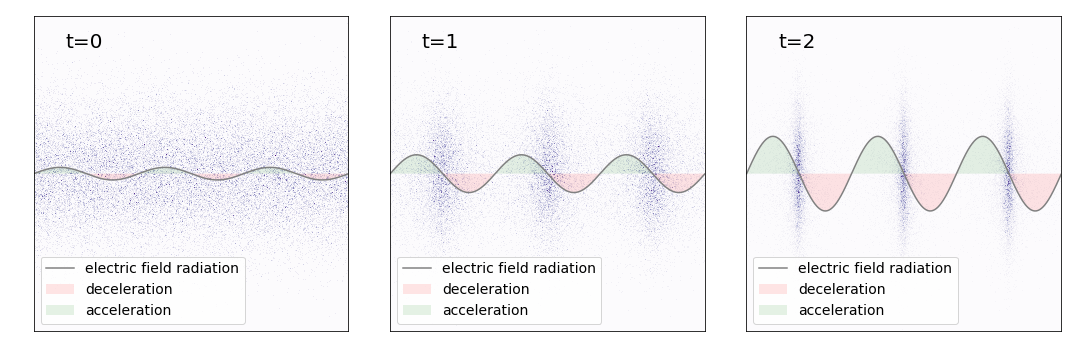
\includegraphics[width=100mm]{Chapter_03_GenerationXrayXFEL_microbunching.png}
\caption{Self-samplified stimulated emission (SASE). The electric field of the radiation will induce an energy modulation within the electron bunch, that results in microbunches. The three panels illustrate that the electric field will induce an energy modulation within the electron bunch. Certain electrons will be accelerated, and others decellerated, as indicated by the green and red areas. This phenomenon is called slippage. As a result the electrons group in microbunches. The modulation amplifies as more and more electrons group together. The amplications will end when all electrons emit in phase.  }\label{fig:microbunching}
\end{figure}